%!TEX root = ../report.tex
\begin{document}
\chapter{Methodology}
In this chapter, we will discuss about RandLA-Net used for 3D semantic segmentation, 
especially about how the RandLA-Net architecture helps in efficient segmentation.
How random point sampling along with local feature aggregation module in RandLA-Net is better than other sampling methods.
We also discuss about the deep ensembles for uncertinty quantification and, we conclude this chapter with the environment and training details for the RandLA-Net with deep ensembles.
\section{RandLA-Net}
As stated in \cite{Hu_2020_CVPR_Randla}, it is a light weight, and efficient neural network architecture for sematic segmentation of 3D point clouds.
From related work section cite here, we can observe that the RandLA-Net architecture is best performing among the point models.
Efficient computation, memory usage and a model with direct application o 3D points are the main motivation when developing the RandLA-Net.
To acheive these goals, RandLA-Net employs random point sampling along with the local feature aggregation module.
Authors in \cite{Hu_2020_CVPR_Randla} proved that by a successive application of random point sampling along with lcoal feature aggregation module effective reduce and extract the features of the large scale point clouds from a scale of $10^5$ to $10^2$.

RandLA-Net utilizes random point sampling among the other sampling methods such as Farthest Point Sampling, Inverse Density Point Sampling.
In random point sampling, we select K points uniformly from original point cloud and has a computational complexity time of O(1).
When compared among other point sampling methods, random point sampling has the lowest computational complexity and computation time is completely independent on number of points.
Despite of these advantages, random point sampling comes with a major disadvantgae of important points being dropped.
To overcome this, authors of RandLA-Net proposed local feature aggragation module for progressive capture of complex features on these selected points.
\begin{figure}
    \centering
    \begin{subfigure}{0.45\textwidth}
        \centering
            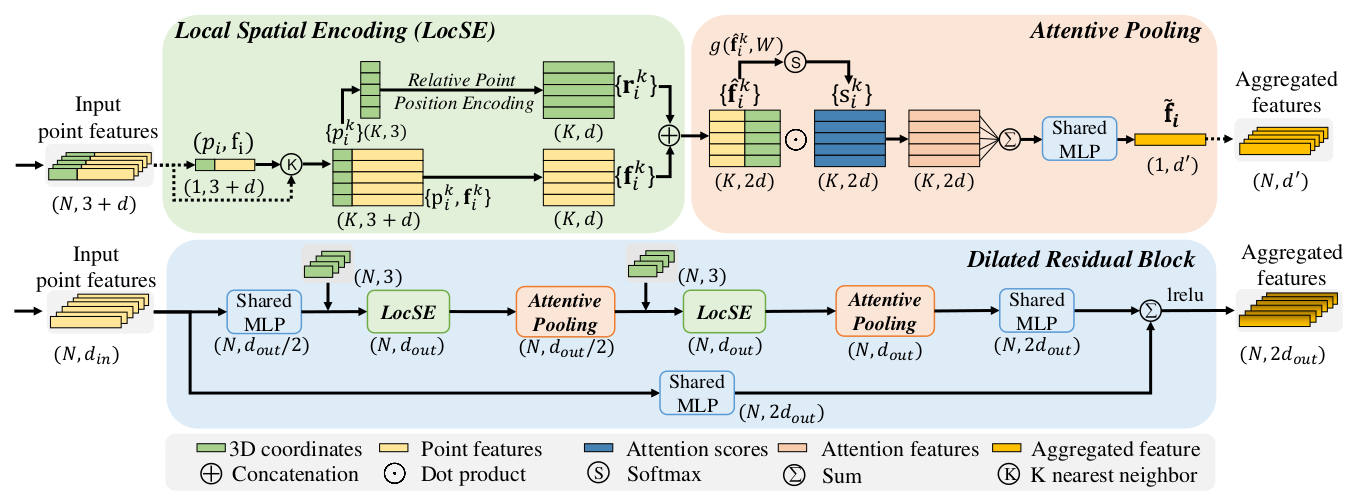
\includegraphics[scale=0.4, angle=90]{images/localfeatueaggregation-randlanet.png}
            \caption{}
            \label{fig:randlanetlfa}       
    \end{subfigure}
    \begin{subfigure}{0.45\textwidth}
        \centering
            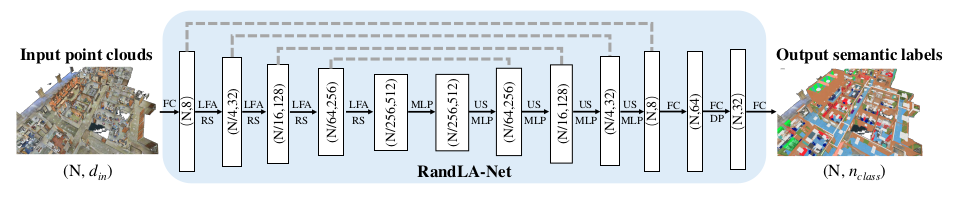
\includegraphics[scale=0.55, angle=90]{images/randlanet.png}
            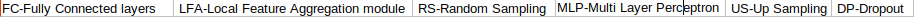
\includegraphics[scale=0.55, angle=90]{images/archi_expl.png}
            \caption{}
            \label{fig:networkarchitecture}
    \end{subfigure}
    \caption{Illustration of (a) local feature aggregation module in RandLa-Net and (b) architecture of RandLA-Net. Both the images are taken from \cite{Hu_2020_CVPR_Randla}}
\end{figure}

Figure \ref{fig:randlanetlfa} represents the local features aggregation module for the RandLA-Net.
This module is applied paralelly on the 3D points and architecture of local feature aggregation module is further divided into three sub modules.
They are local spatial encoding (LocSE), attentive pooling and dilated residual block represented as green, pink and blue blocks respectively in Figure \ref{fig:randlanetlfa}.
Let us discuss further each of these submodules in detail.

\subsection{Local Spatial Encoding (LocSE)}
Local spatial enconding module takes each point ($p_i$) in point cloud (P) and encodes its neighbouring points position(x, y and z).
This encoding makes sure that point p always have information of its neighbours.
Also this encoding helps in learning geometric patterns and learn complex structures progressively.
This module works in three steps:
\begin{enumerate}
    \item Finding nearest neighbours
    \item Relative position encoding
    \item Feature augmentation
\end{enumerate}

In step 1, neighbouring points for point ($p_i$) are collected using euclidean distance based K-nearest neighbour (KNN) algorithm.
Step 2 encodes these collected K-points for point ($p_i$) using a Multi Layer Perceptron (MLP) into realtive point position. The encoding formula is given by
$$
r_i^k = MLP(p_i \oplus p_i^k \oplus (p_i - p_i^k) \oplus ||p_i-p_i^k||)
$$
where $r_i^k$ is the relative position of point $p_i$ with respect to $p_i^k$, here in $p_i$ and $p_i^k$ only the x,y and z positions are used.
$\oplus$, and $||p_i-p_i^k||$ represents the concatenation operation and euclidean distance calculation between $p_i$ and $p_i^k$ respectively.
This step 2 of relative position encoding is represented by above part in LocSE module in green track in Figure \ref{fig:randlanetlfa}.
Step 3 creates a augmented feature vector $\hat{f_i^k}$ by concatenation of relative point position ($r_i^k$) and its point features ($f_i^k$) of point $p_i^k$.
Point features ($f_i^k$) include the R,G and B values and other features such as intensity values.
This step 3 is represented in lower part of the LocSE module in yellow track in Figure \ref{fig:randlanetlfa}.

\subsection{Attentive Pooling}
This augmented feature vector $\hat{f_i^k}$ from LocSE module is passed through a pooling layer to extract important features.
Authors state that use of max and mean pooling layer leads in loss of information, because of this authors made use of attention mechanism which helps in learning important features automatically.
Given the feature vector $\hat{f_i^k}$ a function $g$ is learned by help of MLP and softmax and the resultant vector is denoted as $s_i^k$ in the pink block in Figure \ref{fig:randlanetlfa}.
These each feature score $s_i^k$ from function $g$ is multiplied with feature vector $f_i^k$ called informative feature vector and summed up to form a unique feature vector $\tilde{f_i}$ for point $p_i$ and this operation is mathematically denoted as
$$
\tilde{f_i}= \sum_{k=1}^K (\hat{f_i^k}.s_i^k)
$$

\subsection{Dilated Residual Block}
Dilated Resudial Block is a ResNet inspired module as claimed by authors and represented as blue color module in Figure \ref{fig:randlanetlfa}.
This module is a combination of multiple LocSE, Attentive Polling, and a skip connection which feeds informative feature vector to output.
\begin{figure}
    \centering
    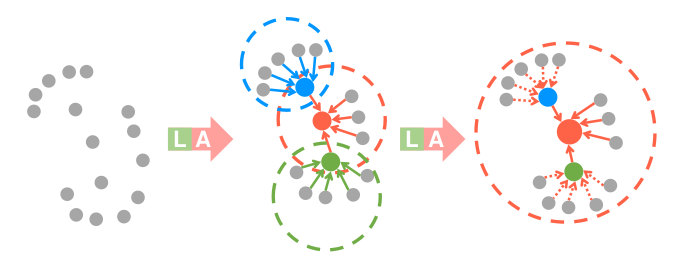
\includegraphics[scale=0.5]{images/dilatedresidualblock.png}
    \caption{Dilated residual block. Image taken from \cite{Hu_2020_CVPR_Randla}.}
    \label{fig:dilatedresidualblock}
\end{figure}
Let us consider a red point in Figure \ref{fig:dilatedresidualblock} and after application of first LocSE and Attentive Pooling module it observes K neighbours represented in red circle.
Secondary application of LocSE and Attentive Polling allows the red point to observe $K^{2}$ neighbours represented as large red circle in right subimage in Figure \ref{fig:dilatedresidualblock}.
This progressive dilation of receptive fields allows to observe local features in first application of LocSe and Attentive Pooling and then observe global features on further application of LocSE and Attentive Polling modules.
Authors claim that more LocSE and Attentive Pooling stacked in Dilated Residual Block powerful the Dilated Residual Block becomes and greater the receptive field at an expense of computational time.
Authors also claim that only by stacked application of two LocSE and Attentive Pooling modules is powerful enough and it is effective and efficient in computational time.

To summarize upto this point, we have studied the special feature of RandLA-Net. That is how random point sampling in conjecture with local features aggregation module in Figure \ref{fig:randlanetlfa} helps in extraction of features progressively.
We also studied how local feature aggragation module is divided into three sub modules namely Local Spatial Encoding (LocSE), Attentive Pooling and Dilated Residual Block and each of this submodules working procedure.
In the next section we study the architecture of RandLA-Net.

\subsection{RandLA-Net architecture}
RandLA-Net is an encoder-decoder architecture with skip connections as used in various segmentation networks such as 3D U-Net\cite{wang2018two_3DUnet}.
The input point clouds are directly applied to encoder consisting of Fully Connected (FC) and four Local Feature Aggragation (LFA) modules connected sequentially.
The size of point cloud reduces by a factor of 4 for every encoder layer. 
Similarly four decoder layers are used and the input features maps to each decoder layer is upsampled and concatenated to respective encoder feature maps via skip connections.
The MLP is applied and fed into next decoder layer.
Output of final decoder layer is fed in to 3 FC layers for point classification and a dropout layer is added before last layer with a dropout rate of 0.5.
The detailed network architecture is illustrated in Figure \ref{fig:networkarchitecture}.


We chose RandLA-Net because of the following reasons:
\begin{enumerate}
    \item Efficient extraction of complex structures progressively using Local Feature Aggregation (LFA) module.
    \item Has lower number of parameters (1.24M) making training efficient, as 3D semantic segmentation models are computationally expensive.
    \item Proven performance over variety of datasets such as Semantic3D and SemanticKITTI, along with ablation study of each submodule in LFA proposed in \cite{Hu_2020_CVPR_Randla}.
    \item No preprocessing such as range image representation as in \cite{Milioto2019} or farthest point sampling with a computaitonal complexity of $O(N^2)$ as in \cite{Qi_2017_CVPR_pointnet}. Whereas RandLA-Net employs random point sampling with computational time of $O(1)$.
    \item State of the art performance in point based methods, consisting of only Multi Layer Perceptrons (MLP) and without expensive operations such as kernalization or graph construction.
\end{enumerate}

Here, we conclude the study of RandLA-Net, reason for its effective performance and argued the reasons to chose RandLA-Net.
In following sections we will discuss about the utilized uncertainty estimation methods such as deep ensembles,......
\section{Deep ensembles}
\end{document}
